\chapter{Authorization}
In this chapter are analyzed all the aspects that build the \textit{authorization} infrastructure in Istio Security. Moreover, a further analysis is done on the policies, ending with an in-depth analysis on the policy enforcement mechanism in order to understand how they are translated in firewall rules to enable/disable the communications between services.
\minitoc

\section{Architecture}
Istio Security gives the possibility to perform authorization for workload-to-workload and user-to-workload. Moreover, it supports any TCP protocols, in particular HTTP, HTTPS and gRPC. It is flexible, since custom conditions can be defined on Istio attributes and it uses only a single and simple API (\texttt{AuthorizationPolicy}) to store the policies and enforce the authorizations directly on the Envoy proxies.
In Fig.~\ref{fig:archauthz} a schematic description of the general authorization architecture is shown.

\begin{figure}[ht]
    \centering
    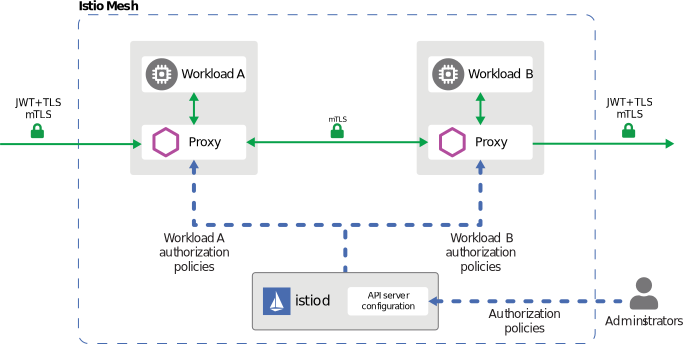
\includegraphics[width=0.9\textwidth]{chapters/images/chp3/arch-authz.png}
    \caption{Istio Security's authorization architecture, from Istio Docs}
    \label{fig:archauthz}
\end{figure}

More in details, once that an administrator applies an authorization policy (using the API server provided by \texttt{istiod}), the policy is split and sent to the interested workload. Here, Envoy takes the policy and runs an authorization controller that, based on the future request, evaluates the context with the policy and \texttt{DENY} or \texttt{ALLOW} the authorization. If no authorization policy is available for a particular workload, then the access control is disabled and all the requests are accepted. For multiple \texttt{AuthorizationPolicy}, the \texttt{DENY} takes precedence over the \texttt{ALLOW} and the specified policies are added by preserving the previously added ones (additively).

\section{Policies}
As already mentioned, the only way of defining custom policies is through the Istio API by using the \texttt{AuthorizationPolicy} kind in the \texttt{.yaml}. As an example, the following policy is chosen:

\begin{lstlisting}
apiVersion: security.istio.io/v1beta1
kind: AuthorizationPolicy
metadata:
 name: httpbin
 namespace: foo
spec:
 selector:
   matchLabels:
     app: httpbin
     version: v1
 action: ALLOW
 rules:
 - from:
   - source:
       principals: ["cluster.local/ns/default/sa/sleep"]
   - source:
       namespaces: ["dev"]
   to:
   - operation:
       methods: ["GET"]
   when:
   - key: request.auth.claims[iss]
     values: ["https://accounts.google.com"]
\end{lstlisting}

\noindent This policy allows two sources (\texttt{cluster.local/ns/default/sa/sleep} service account and \texttt{dev} namespace) to access the workloads by using the \texttt{httpbin} app \texttt{v1} in the namespace \texttt{foo} when a JWT valid Token is used.

\noindent From this example can be extrapolated the structure of the text file:

\begin{itemize}
 \item \texttt{selector}: the target of the policy. In this example is everything that matches \texttt{httpbin} and has version \texttt{v1}.
 \item \texttt{action}: \texttt{ALLOW} or \texttt{DENY}.
 \item \texttt{rules}: when the action is triggered. Furthermore, other keywords are defined, such as \texttt{from} (to specify the source), \texttt{to} (for specifying the operations) and \texttt{when} (to specify the conditions needed).
\end{itemize}

In order to ensure that an allow policy won't bypass a deny one, the Envoy engine checks and evaluates first the deny ones. As another example, it can be added another policy that denies every access that is not from the namespace \texttt{foo}:

\begin{lstlisting}
apiVersion: security.istio.io/v1beta1
kind: AuthorizationPolicy
metadata:
 name: httpbin-deny
 namespace: foo
spec:
 selector:
   matchLabels:
     app: httpbin
     version: v1
 action: DENY
 rules:
 - from:
   - source:
       notNamespaces: ["foo"]
\end{lstlisting}

\noindent This second policy will be literally "added" to the first one, but since it is a deny policy it will be applied first. The resulting policy will be the intersection of the previously applied ones: as a result, only the source from namespace \texttt{foo} is allowed. 

Moreover, Istio allows custom conditions by using \texttt{when} in combination with the \texttt{key} values\footnote{See \url{https://istio.io/latest/docs/reference/config/security/conditions/}} that can be compatible with HTTP, TCP or both of them. For example, the policy can match only defined IP addresses in TCP or HTTP by using \texttt{source.ip} or even match in HTTP only a defined JWT Token value, for example the audience (\texttt{request.auth.audiences}).

\section{Weak points analysis}